\section{Ejercicio Adicional: Oscilador de 12 kHz}
\label{sec_5}
La consigna pide diseñar un oscilador de $f = 12 \, [kHz]$ con capacitores, resistores, una fuente de $\pm 12 \, [V]$ y un LM324, y ajustarlo en simulación a una tolerancia de $\pm 100 \, [Hz]$.

\subsection{Oscilador Puente de Wien}
\label{sec_5.1}
Se adopta el oscilador puente de Wien \cite[sec.~8.1]{apuntes8} de la \autoref{fig:wien}: un amplificador no inversor de ganancia $A = 1 + R_f/R_g$ realimentado positivamente a través de una red $RC$ serie--paralelo. Con $R_1 = R_2 = R$ y $C_1 = C_2 = C$, la transferencia de la red es
\begin{equation}
    \beta(j\omega) = \frac{V_p}{V_{out}} = \frac{1}{3 + j\left(\dfrac{\omega}{\omega_0} - \dfrac{\omega_0}{\omega}\right)}, \qquad \omega_0 = \frac{1}{RC}
    \label{eq:wien}
\end{equation}
A la frecuencia $\omega_0$ la red no desfasa y atenúa $1/3$, de modo que por el criterio de Barkhausen ($A\beta = 1$) el circuito oscila en
\begin{equation}
    f_0 = \frac{1}{2 \pi R C} \qquad \text{con} \qquad A = 1 + \frac{R_f}{R_g} = 3
\end{equation}

\begin{figure}[H]
    \centering
    \begin{circuitikz}[scale=0.8, transform shape]
        \draw (0,0) node[op amp, noinv input up] (U) {$U_1$};
        \draw (U.+) -- ++(-1,0) coordinate (P) node[above right]{$V_p$};
        \draw (P) -- ++(0,2) coordinate (T) to[R, l=$R_1$, a=$8.25 \, k\Omega$] ++(2.6,0) to[C, l=$C_1$, a=$1.5 \, nF$] ++(2.6,0) coordinate (T2);
        \draw (P) -- ++(-1.5,0) coordinate (P2) to[R, l_=$R_2$, a^=$8.25 \, k\Omega$, *-] ++(0,-2.5) node[ground]{};
        \draw (P2) -- ++(-3,0) to[C, l_=$C_2$, a^=$1.5 \, nF$] ++(0,-2.5) node[ground]{};
        \draw (U.-) -- ++(-0.5,0) coordinate (N) -- ++(0,-1.5) coordinate (N2);
        \draw (N2) to[R, l_=$R_g$, a^=$10 \, k\Omega$, *-] ++(0,-2) node[ground]{};
        \draw (N2) to[R, l=$R_{f1}$, a=$15 \, k\Omega$] ++(2.4,0) coordinate (M) to[R, l=$R_{f2}$, a=$6.8 \, k\Omega$, *-*] ++(2.4,0) coordinate (M2);
        \draw (M) -- ++(0,-1.4) to[D, l_=$D_1$] ($(M2)+(0,-1.4)$) -- (M2);
        \draw ($(M)+(0,-1.4)$) -- ++(0,-1.4) to[D, l_=$D_2$, invert] ($(M2)+(0,-2.8)$) -- ($(M2)+(0,-1.4)$);
        \draw (U.out) -- (U.out -| T2) node[circ]{} to[short, -o] ++(1,0) node[right]{$V_{out}$};
        \draw (T2) -- (M2);
    \end{circuitikz}
    \caption{Oscilador puente de Wien con control de amplitud por diodos ($D_1$, $D_2$: 1N4148; LM324 con $\pm 12 \, [V]$).}
    \label{fig:wien}
\end{figure}

\subsection{Control de Amplitud y Límite por Slew Rate}
\label{sec_5.2}
Para que la oscilación arranque, la ganancia inicial debe superar levemente a $3$; si se mantuviera constante, la amplitud crecería hasta saturar el amplificador. Por eso la resistencia de realimentación se divide en $R_{f1}$ y $R_{f2}$, y sobre $R_{f2}$ se colocan dos diodos en antiparalelo. Con señal pequeña los diodos no conducen y
\begin{equation}
    A_0 = 1 + \frac{R_{f1} + R_{f2}}{R_g} = 1 + \frac{15 + 6.8}{10} = 3.18
\end{equation}
un $6 \, [\%]$ por encima del valor crítico. Al crecer la amplitud, los diodos conducen en los picos y reducen la resistencia equivalente de $R_{f2}$ hasta que la ganancia efectiva vale $3$, es decir, hasta que $R_{f2,ef} = 2R_g - R_{f1} = 5 \, [k\Omega]$. En esa condición la tensión sobre $R_{f2}$ es del orden de la de conducción de los diodos ($V_D \approx 0.5 \, [V]$), y como la corriente de la rama es $V_{out}/(3R_g)$:
\begin{equation}
    V_{out,p} \approx V_D \, \frac{3 R_g}{R_{f2,ef}} = 0.5 \, [V] \cdot \frac{30 \, [k\Omega]}{5 \, [k\Omega]} = 3 \, [V]
    \label{eq:amplitud}
\end{equation}

La amplitud debe quedar además por debajo de la que permite el \textit{slew rate} del LM324 ($0.5 \, [V/\mu s]$ típico \cite[sec.~6.10]{lm324}) a $12 \, [kHz]$:
\begin{equation}
    V_{max} = \frac{SR}{2 \pi f_0} = \frac{0.5 \, [V/\mu s]}{2 \pi \cdot 12 \, [kHz]} = 6.6 \, [V]
\end{equation}

\subsection{Ajuste de la Frecuencia}
\label{sec_5.3}
Con $C = 1.5 \, [nF]$, el valor teórico es $R = 1/(2\pi \cdot 12 \, [kHz] \cdot 1.5 \, [nF]) = 8.84 \, [k\Omega]$. Sin embargo, el LM324 ($GBW = 1 \, [MHz]$ en el macromodelo utilizado; $1.2 \, [MHz]$ típico según la hoja de datos \cite[sec.~6.10]{lm324}) configurado con ganancia $3$ tiene un ancho de banda de unos $333 \, [kHz]$ e introduce un retardo de fase de aproximadamente $2^\circ$ a $12 \, [kHz]$. Como señalan los apuntes de la cátedra \cite[sec.~8.1]{apuntes8}, el desfasaje del polo del amplificador comienza a notarse una década antes de ese polo; si la frecuencia de oscilación cae en esa zona, la red $RC$ debe compensarlo para satisfacer la condición de fase, y la oscilación se produce a una frecuencia menor que la ideal. En la red de Wien, esa compensación solo ocurre por debajo de $\omega_0$ (\autoref{eq:wien}). Como la pendiente de fase de la red en $\omega_0$ es de $-2/3 \, [rad]$ por unidad de frecuencia normalizada, el corrimiento esperado es de aproximadamente $5 \, [\%]$.

Para ajustar la frecuencia se simuló el circuito con los valores de la serie E96 entre $7.87$ y $9.09 \, [k\Omega]$, midiendo la frecuencia sobre $200$ ciclos de régimen permanente (\autoref{tab:ajuste_osc} y \autoref{fig:osc_ajuste}).

\begin{table}[H]
    \centering
    \caption{Barrido de $R$ ($C = 1.5 \, [nF]$, LM324).}
    \label{tab:ajuste_osc}
    \begin{tabular}{|c|c|c|c|}
        \hline
        $\boldsymbol{R}$ & $\boldsymbol{f_{osc}}$ \textbf{simulada} & \textbf{Error respecto de 12 kHz} & \textbf{THD} \\
        \hline
        $7.87 \, [k\Omega]$ & $12590.9 \, [Hz]$ & $+590.9 \, [Hz]$ & $2.98 \, [\%]$ \\
        $8.06 \, [k\Omega]$ & $12310.8 \, [Hz]$ & $+310.8 \, [Hz]$ & $2.98 \, [\%]$ \\
        $\mathbf{8.25 \, [k\Omega]}$ & $\mathbf{12042.6 \, [Hz]}$ & $\mathbf{+42.6 \, [Hz]}$ & $\mathbf{2.99 \, [\%]}$ \\
        $8.45 \, [k\Omega]$ & $11772.8 \, [Hz]$ & $-227.2 \, [Hz]$ & $3.00 \, [\%]$ \\
        $8.66 \, [k\Omega]$ & $11502.1 \, [Hz]$ & $-497.9 \, [Hz]$ & $3.00 \, [\%]$ \\
        $8.87 \, [k\Omega]$ & $11243.7 \, [Hz]$ & $-756.3 \, [Hz]$ & $3.01 \, [\%]$ \\
        $9.09 \, [k\Omega]$ & $10985.2 \, [Hz]$ & $-1014.8 \, [Hz]$ & $3.01 \, [\%]$ \\
        \hline
    \end{tabular}
\end{table}

\begin{figure}[H]
    \centering
    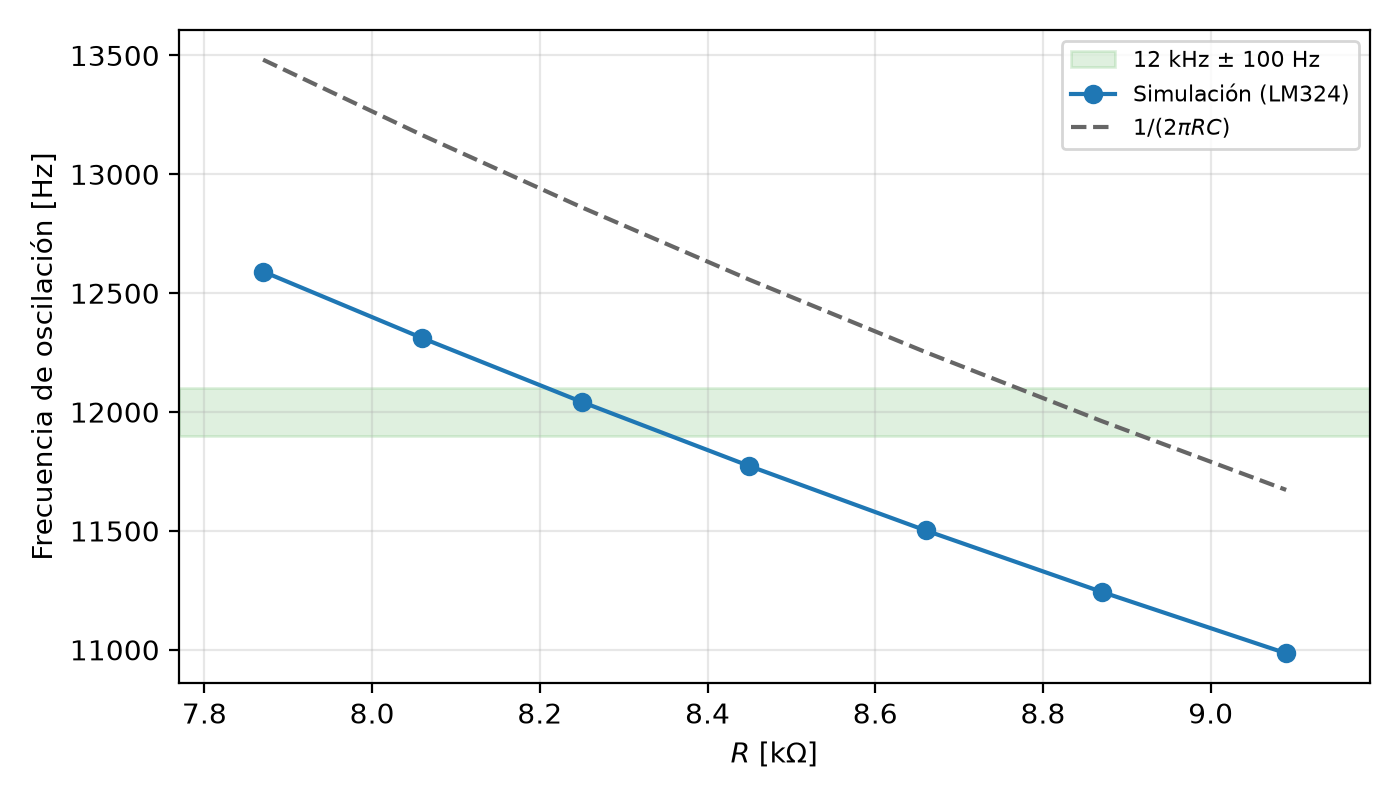
\includegraphics[width=0.7\textwidth]{osc_ajuste_R.png}
    \caption{Frecuencia de oscilación en función de $R$, simulada y teórica.}
    \label{fig:osc_ajuste}
\end{figure}

Con el valor teórico ($8.87 \, [k\Omega]$ en la serie E96) el circuito oscila en $11244 \, [Hz]$, un $6 \, [\%]$ por debajo de lo esperado, como anticipaba el análisis de fase. Se adopta $R = 8.25 \, [k\Omega]$, con el que la frecuencia resulta $12042.6 \, [Hz]$, dentro de la tolerancia de $\pm 100 \, [Hz]$.

\subsection{Simulación}
\label{sec_5.4}
El circuito se simuló con el macromodelo \texttt{LM324/NS} y diodos 1N4148, partiendo de una condición inicial de $10 \, [mV]$ en la entrada no inversora. La oscilación crece y se estabiliza en menos de $1 \, [ms]$ (\autoref{fig:osc_arranque}).

\begin{figure}[H]
    \centering
    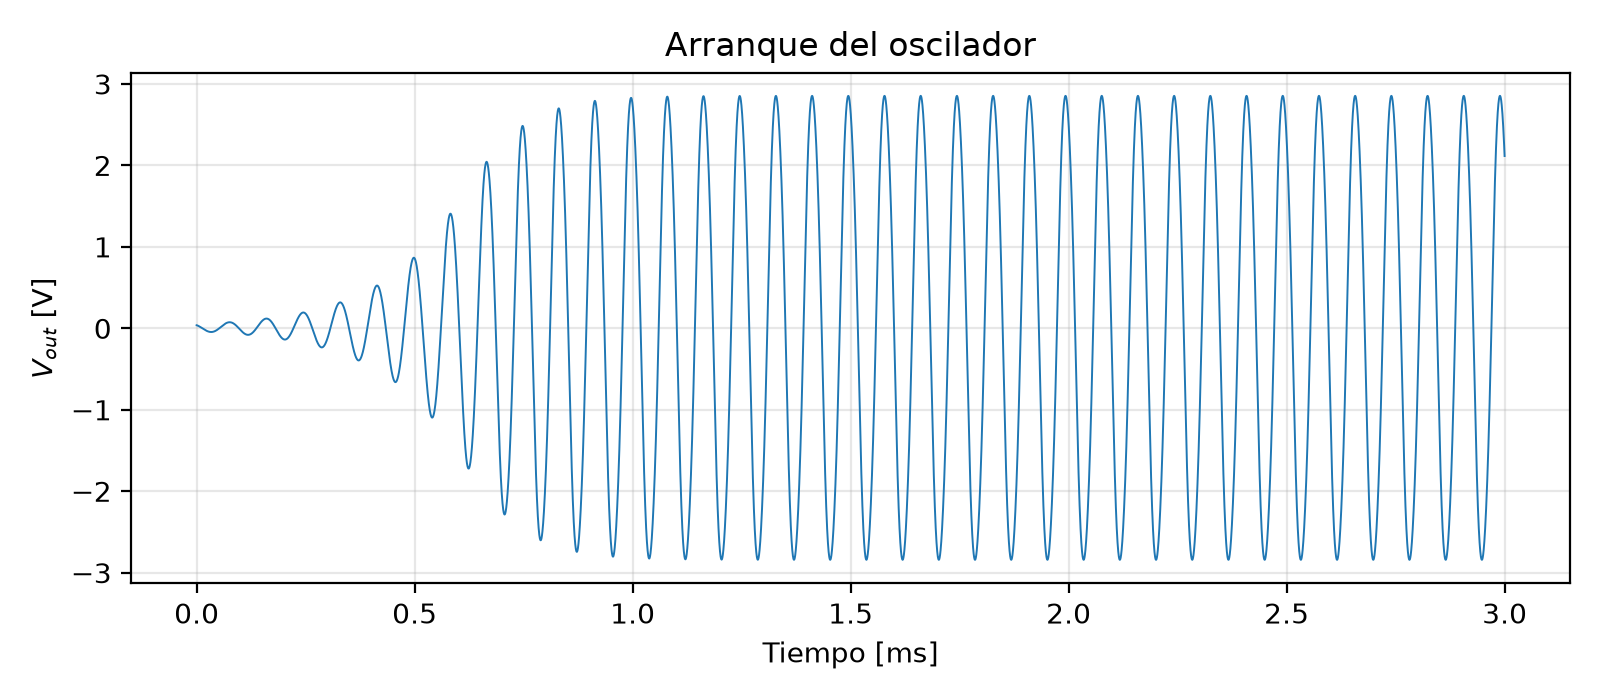
\includegraphics[width=0.8\textwidth]{osc_arranque.png}
    \caption{Arranque del oscilador.}
    \label{fig:osc_arranque}
\end{figure}

\begin{figure}[H]
    \centering
    \begin{subfigure}{0.49\textwidth}
        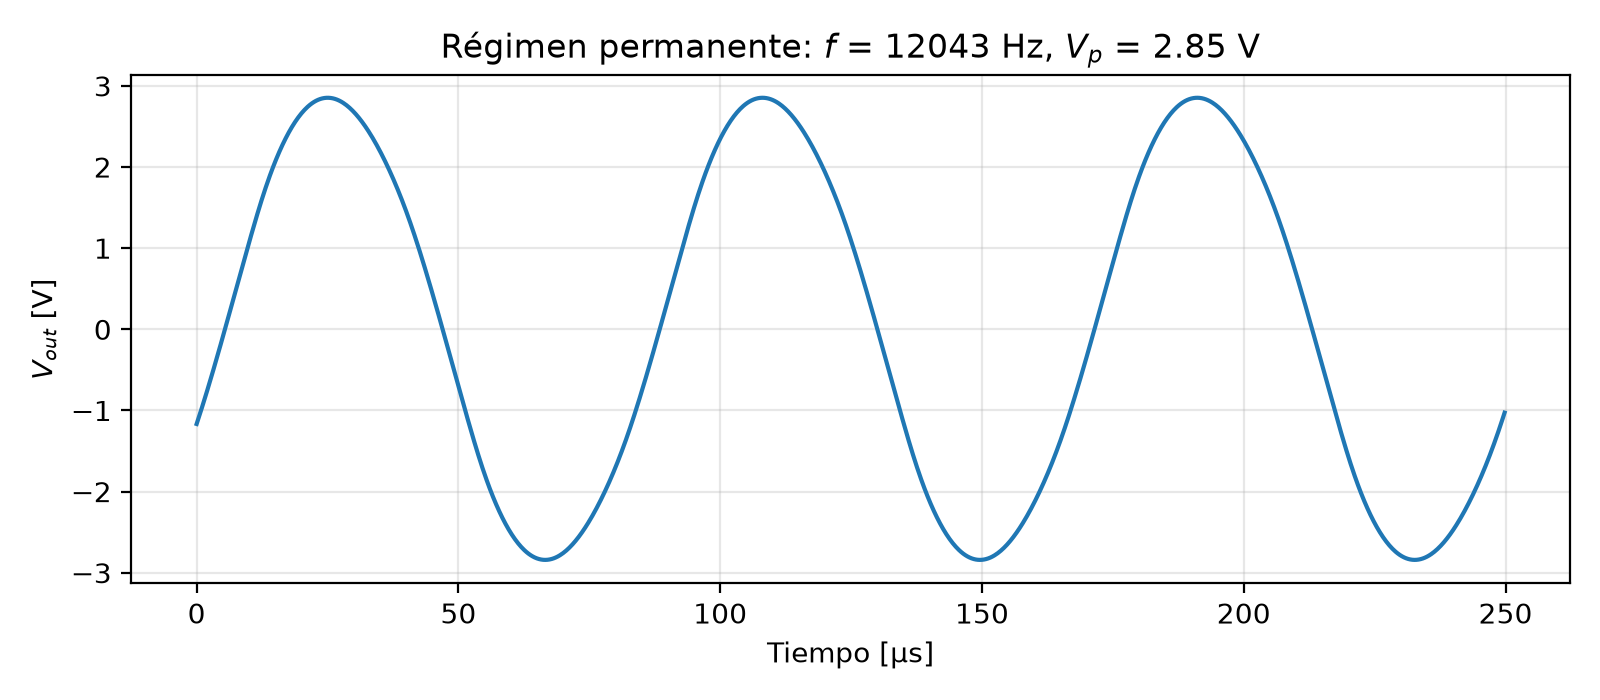
\includegraphics[width=\textwidth]{osc_permanente.png}
        \caption{Régimen permanente.}
        \label{fig:osc_perm}
    \end{subfigure}
    \hfill
    \begin{subfigure}{0.49\textwidth}
        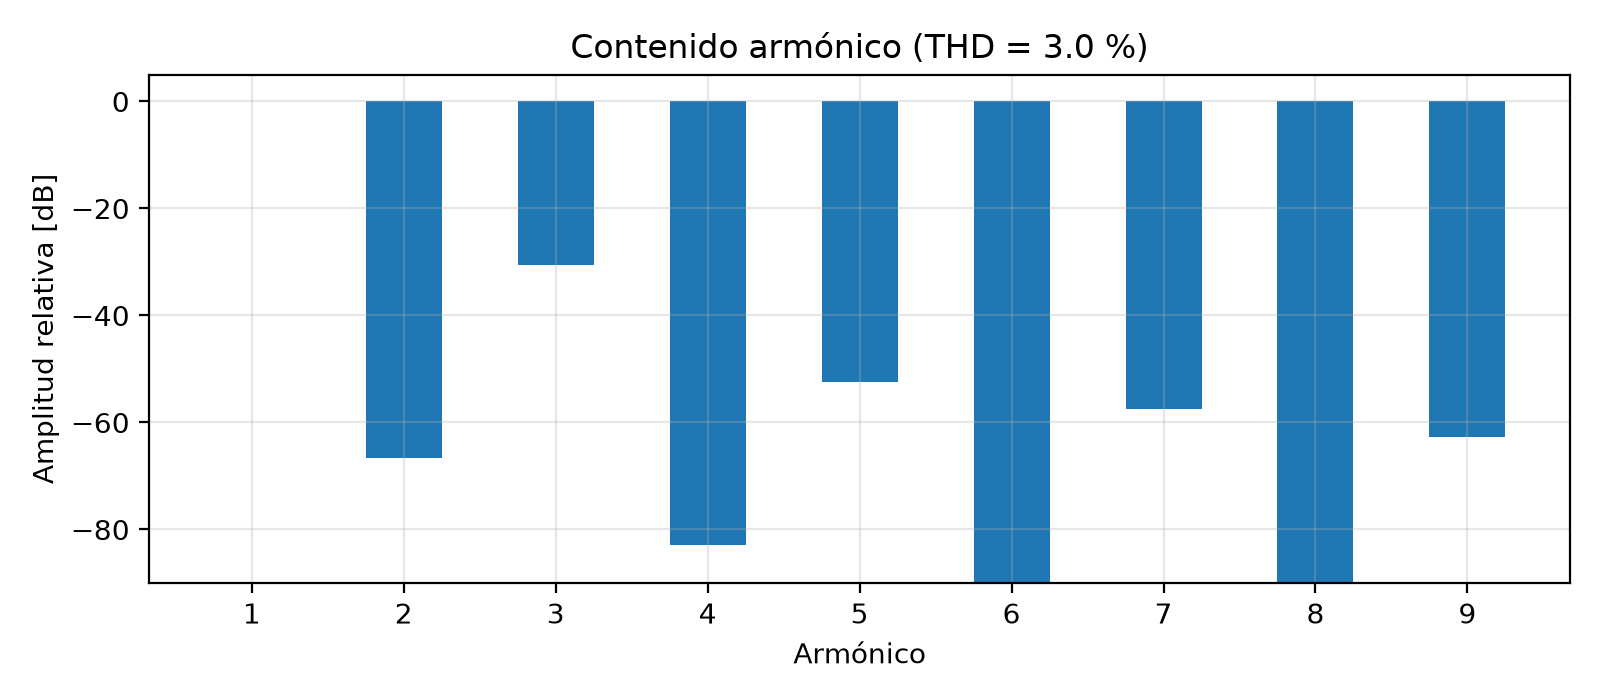
\includegraphics[width=\textwidth]{osc_espectro.png}
        \caption{Contenido armónico.}
        \label{fig:osc_espectro}
    \end{subfigure}
    \caption{Tensión de salida en régimen permanente.}
\end{figure}

En régimen permanente la amplitud es de $2.85 \, [V]$ de pico, en acuerdo con la estimación de la \autoref{eq:amplitud}. La distorsión armónica total, calculada sobre $9$ armónicos mediante un ajuste por mínimos cuadrados sobre los últimos $10 \, [ms]$, es del $3.0 \, [\%]$, dominada por el tercer armónico ($-30.5 \, [dB]$), como corresponde a la alinealidad simétrica de los diodos.

\begin{table}[H]
    \centering
    \caption{Resultados del oscilador.}
    \label{tab:osc}
    \begin{tabular}{|l|c|}
        \hline
        \textbf{Parámetro} & \textbf{Valor} \\
        \hline
        Frecuencia de oscilación & $12042.6 \, [Hz]$ ($+0.35 \, [\%]$) \\
        Amplitud de salida & $2.85 \, [V]$ de pico \\
        Distorsión armónica total & $3.0 \, [\%]$ \\
        Tiempo de establecimiento & $< 1 \, [ms]$ \\
        \hline
    \end{tabular}
\end{table}

\subsection{Verificación del Límite por Slew Rate}
\label{sec_5.5}
Para mostrar por qué la amplitud debe limitarse, se simuló el circuito con $R_{f1} = 18 \, [k\Omega]$ y $R_{f2} = 4.7 \, [k\Omega]$, que llevan $R_{f2,ef}$ a $2 \, [k\Omega]$ y la amplitud prevista por la \autoref{eq:amplitud} a unos $7.5 \, [V]$. La simulación da $7.54 \, [V]$ de pico. La \autoref{fig:osc_slew} compara ambas versiones junto con la derivada de la salida: con la red elegida la pendiente máxima es de $0.23 \, [V/\mu s]$, mientras que con la red alternativa la derivada se aplana en $\pm 0.49 \, [V/\mu s]$ cerca de los cruces por cero, es decir, el amplificador trabaja a su velocidad máxima.

\begin{figure}[H]
    \centering
    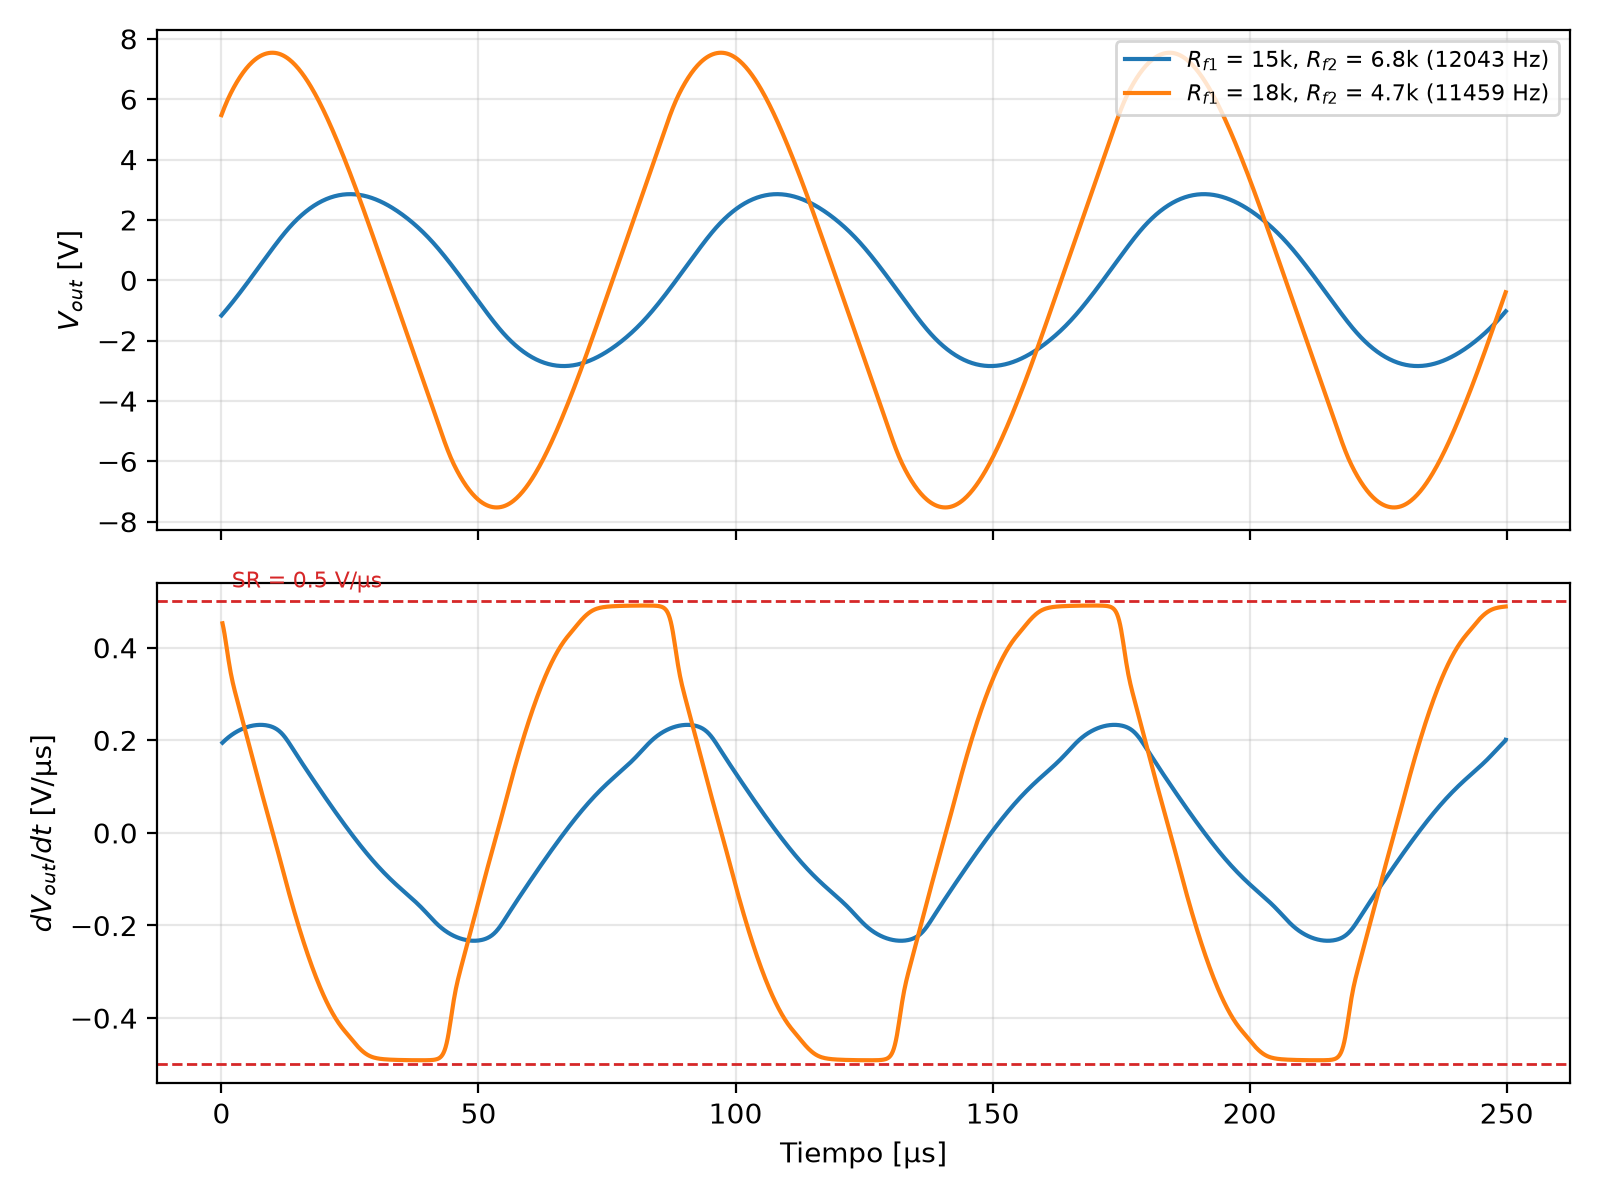
\includegraphics[width=0.8\textwidth]{osc_slew_rate.png}
    \caption{Salida y derivada de la salida para las dos redes de control de amplitud.}
    \label{fig:osc_slew}
\end{figure}

Como la senoidal de $7.54 \, [V]$ requeriría $2\pi \cdot 11.46 \, [kHz] \cdot 7.54 \, [V] = 0.54 \, [V/\mu s]$, apenas un $8 \, [\%]$ más que el \textit{slew rate}, la forma de onda se deforma poco a simple vista. El efecto principal es sobre la frecuencia: el retardo adicional la hace caer a $11459 \, [Hz]$, $584 \, [Hz]$ por debajo del diseño y fuera de la tolerancia pedida.

\subsection{Sensibilidad a las Tolerancias}
\label{sec_5.6}
Como $f_0 \propto (R_1 R_2 C_1 C_2)^{-1/2}$, la sensibilidad de la frecuencia respecto de cada elemento de la red es $-1/2$. Para estimar su efecto se realizó un Montecarlo de $100$ corridas con resistores del $1 \, [\%]$ y capacitores del $5 \, [\%]$ (\autoref{fig:osc_mc}). La frecuencia resultó de $12031 \pm 239 \, [Hz]$ (entre $11546$ y $12645 \, [Hz]$), y solo el $30 \, [\%]$ de los circuitos quedó dentro de $\pm 100 \, [Hz]$.

\begin{figure}[H]
    \centering
    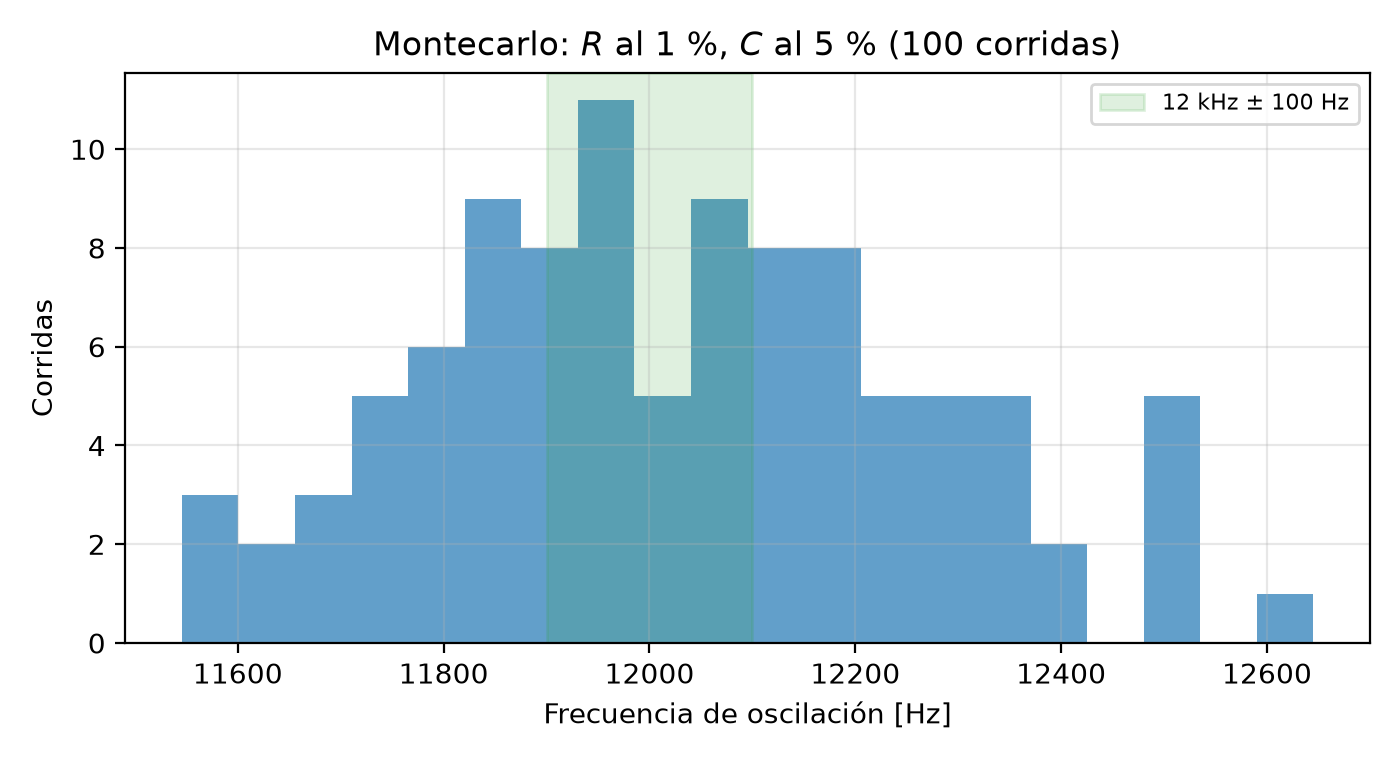
\includegraphics[width=0.7\textwidth]{osc_montecarlo.png}
    \caption{Distribución de la frecuencia de oscilación con $R$ al $1 \, [\%]$ y $C$ al $5 \, [\%]$.}
    \label{fig:osc_mc}
\end{figure}

Por lo tanto, en una implementación física es necesario un elemento de ajuste, por ejemplo reemplazar $R_2$ por una resistencia de $7.5 \, [k\Omega]$ en serie con un preset de $1 \, [k\Omega]$. La variación de $R_2$ altera levemente la atenuación de la red, pero el lazo de control de amplitud lo compensa.
